\chapter{Data Preparation and Processing}
\label{chapter:data_prep_and_proc}
The data volume of interferometric measurements inherently scale as the square of the number of antennas in the array ($N_{\rm ant}$). Not only does the sheer volume of data from large-$N_{\rm ant}$ arrays pose a problem for data storage, but also it requires precise and efficient efforts to quality assure (QA) the data. 

In this chapter, I will outline some of the efforts involved in data preparation, preprocessing and QA that are required for an EoR power spectrum estimate.

\section{Data Compression}
\label{sec:data_compression}

The PAPER-128 correlator produced 288 {\sc miriad} files per night. Each of these contained 8126 baselines, and each baseline contained visibilities over 1024 $98$\,kHz frequency channels and 56 $10$\,s time integrations. The four instrumental polarizations were in separate files. In sum, each file was 4.2 GB which meant that each night 1.2 TB of data were recorded.

In order to efficiently transport the data over Gigabit Ethernet from the Karoo Radio Quiet Zone (KRQZ) to Cape Town, and from Cape Town under transatlantic cables to Philadelphia, some compression was required. It was also required that such a compression, while lossy, did not effect the targeted cosmological signal.

\subsection{Delay--Delay-Rate Filtering}

The compression algorithm implemented for PAPER observations, Delay--Delay-Rate (DDR) filtering, was introduced in \cite{ParsonsBacker.09} described in \cite{Parsons.14}, and we briefly review it below.

The geometric delay of a celestial signal, originating form direction $\hat{s}$, incident on an interferometric baseline described by vector $\vec{b}$, is

\begin{equation}
\tau_g = |\vec{b} \cdot \hat{s}|/c
\end{equation}

where $c$ is the speed of light. This relationship implies that $\tau_g$ is bounded for a given baseline

\begin{equation}
- |\vec{b}|/c \leqslant \tau_g \leqslant |\vec{b}|/c
\label{eq:geometric_delay_bound}
\end{equation}

Equation~\ref{eq:geometric_delay_bound} therefore gives the maximum value of $|\tau_g|$ physically meaningful for a given array -- the maximum baseline length in that array, divided by $c$. For PAPER, the maximum baseline length is 300\,m, corresponding to $\max(|\tau_g|) = 1\mu$s. 
As reviewed in Chapter~\ref{chapter:eor_window_theory}, the delay axis may be accessed by Fourier transforming a visibility along the frequency axis. Once in delay space, power at delays larger in magnitude than $1 \mu$s could be removed. With a sufficiently large frequency bandwidth, this would not produce aliased signal, according to the critical Nyquist rate. By using the $1 \mu$s as a delay bound for all visibilities, the frequency axes of all compressed visibilities remained the same (reduced in number from 1024 to 203), which while sub-optimal from a compression point of view, allowed for ease of programming at later stages.

A similar geometric bound can be obtained by Fourier transforming the time axis of visibilities, provided that they were obtained in drift-scan mode (see Chapter~\ref{chapter:interferometry}). \cite{ParsonsBacker.09} showed that the rate at which the geometric delay on an interferometric baseline changes is governed only by the position of the array on Earth, and the Earth's rotation:

\begin{equation}
\dot{\tau}_g = -\frac{\omega_{\Earth} \cos\delta}{c} \left( b_x\sin\alpha + b_y\cos\alpha\right)
\end{equation}

where $\omega_{\Earth}$ is the angular frequency of the Earth's rotation, $\alpha$ and $\delta$ are the hour-angle and declination of a point on the celestial sphere, respectively, and $\vec{b}=(b_x,b_y,b_z)$ is the baseline vector expressed in equatorial coordinates.

For arrays not close to the geographic poles, $|b_y| \gg |b_x|$, there is a maximum rate of change (corresponding to ($\alpha$, $\delta$) = (0, 0)), producing a bound on $\dot{\tau}_g$:

\begin{equation}
- \omega_{\Earth}|b_y|/c \leqslant \dot{\tau}_g\leqslant \omega_{\Earth} |b_y|/c
\label{eq:geometric_delay_rate_bound}
\end{equation}

for a 300\,m East-West baseline, the maximum delay-rate is approximately $\max(|\dot{\tau}_g|) = 0.07$\,ns\,s$^{-1}$. This delay-rate was not Nyquist sampled by a single PAPER file: requiring the previous and next files generated for that polarization to be appended on either side of each visibility's time axis to prevent aliasing from the decimation. For the large scale processing of months of data, this required a software pipeline described in Section~\ref{subsec:compression_software}.

There are also other issues with DDR compression, largely associated with instrument systematics. Delay transforms rely on the fact that the bright foregrounds that dominate the measured signal are spectrally smooth, and that the frequency response of the instrument is also spectrally smooth: this of course is the basis for the EoR window paradigm reviewed in Chapter~\ref{chapter:eor_window_theory}. Likewise, delay-rate filtering assumes temporal smoothness. Radio Frequency Interference (RFI) signals created by human communications violate both models of smoothness, since they are typically confined to narrow bandwidths (creating sharp spikes along the frequency axis) and may be transient (creating sharp spikes along the time axis). This requires steadfast identification and flagging algorithms for RFI (see Section~\ref{sec:RFI}), and some variety of interpolation, fitting, or CLEANing across the flagged regions prior to compression.

\subsection{Software Implementation}
\label{subsec:compression_software}

The first season of PAPER-128 data, due to a variety of circumstances, required compression on the computing cluster at the University of Pennsylvania. The raw data were stored on a high-volume drive that was able to connect with the cluster via a low-speed switch. The hardware capable of performing any sort of high-performance processing (i.e. holding the data in RAM) were ten ``compute nodes" connected to the cluster via a high-speed switch, and mounted in an NFS architecture. The compute nodes could only hold $\sim 10$ PAPER-128 files in storage. 

The processing stages for compression of a night of PAPER data, described below, required knowledge of the location and compression state of not only individual files, but also the neighbors-in-time of the file in question, in order to implement the DDR filter described above. To supervise the compression we created a MySQL database, which we interacted with via Shell and Python scripts. The database contained a table for the data files under processing and their compression state, a table of neighbor-relations, a table of file details, and a table of the processing nodes available. The schema of this database is shown in Figure~\ref{fig:database_schema}.

\begin{figure}[h]
\centering
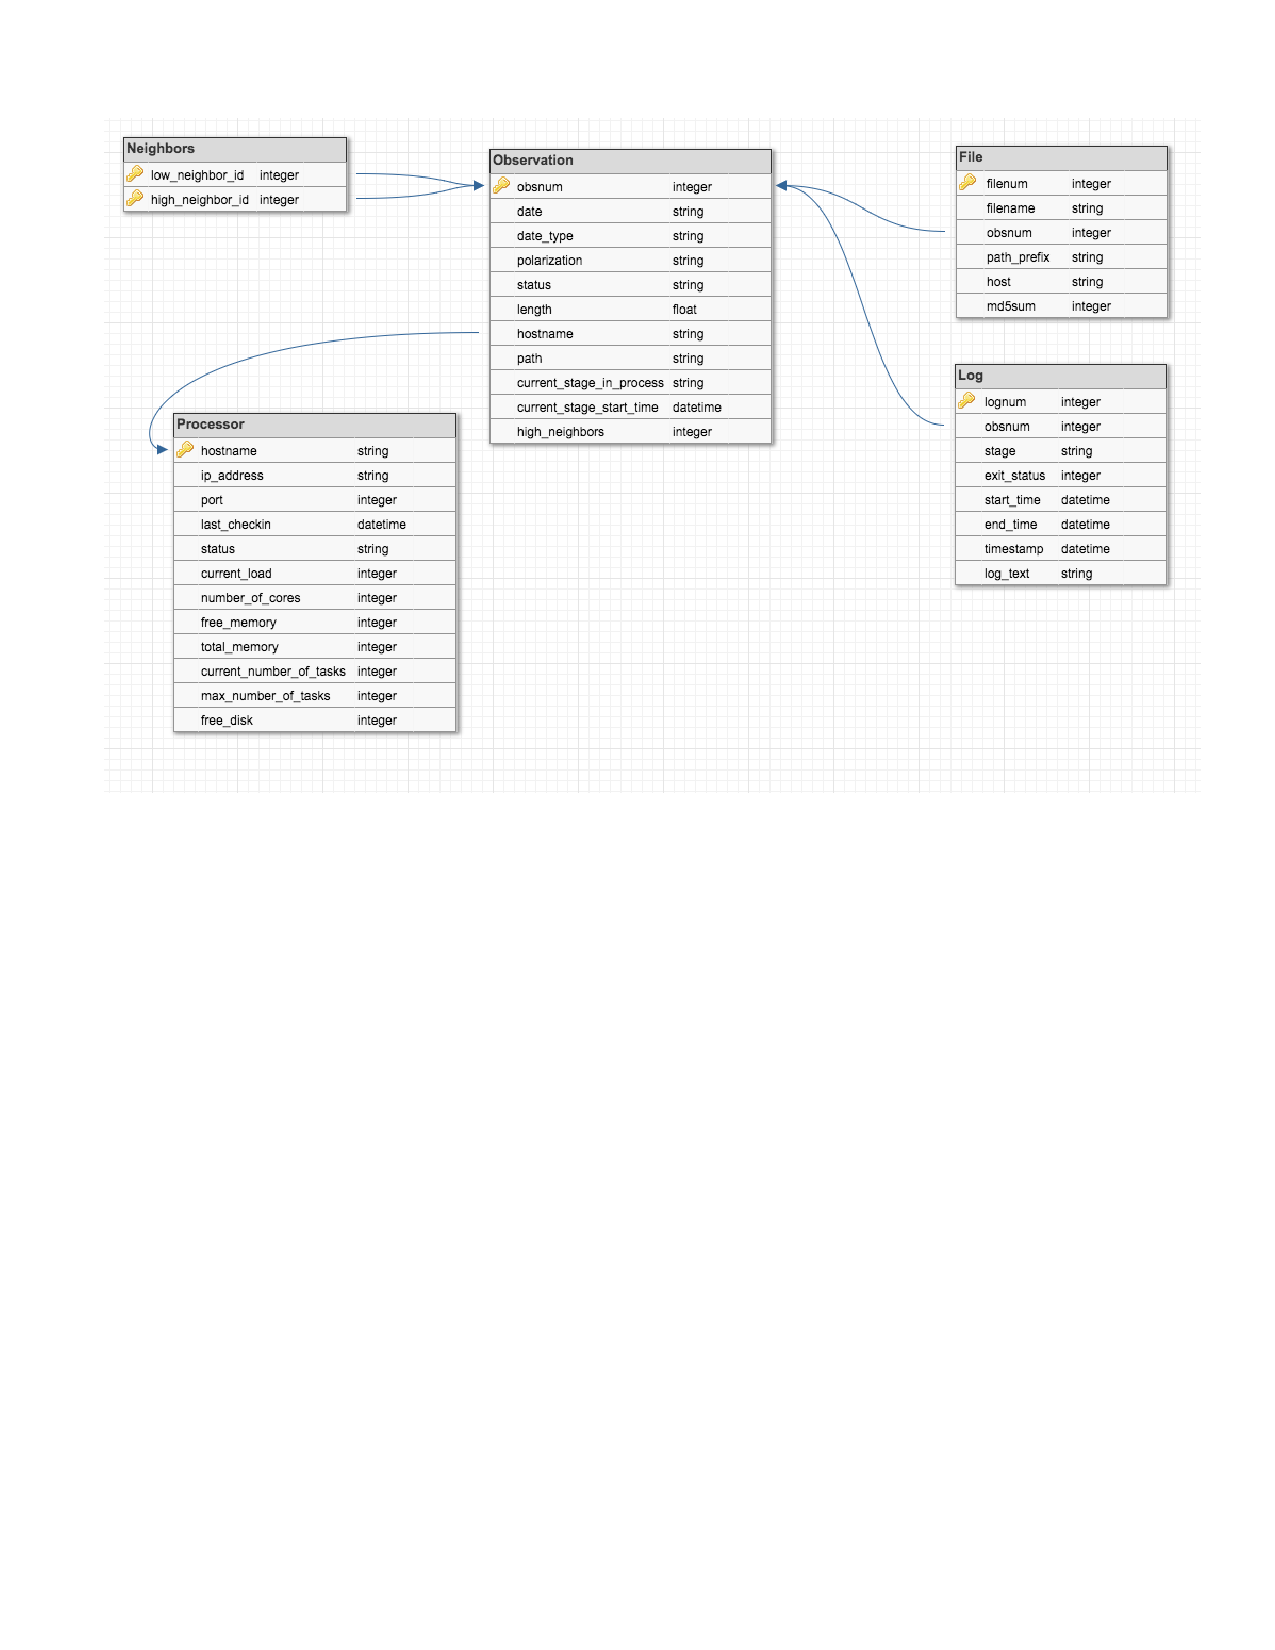
\includegraphics[scale=0.7]{/Users/saulkohn/Documents/thesis/figures/RTP_diagram.pdf}
\caption{The schema of the database used to organize and implement PAPER data compression}
\label{fig:database_schema}
\end{figure}

To implement the compression, per file, the following steps were required:

\begin{enumerate}
\item Copying the file from the storage volume to the cluster. For a single night of data, this required roughly 8 hours.
\item Copying the file from the cluster to the compute node. This required roughly 5 minutes.
\item Generate copy of the file, with metadata corrections. This required roughly 1 minute.
\item Delete the raw file.
\item RFI-flag the high frequency-resolution data. This required roughly 2 minutes.
\item Delete the metadata-corrected file.
\item Acquire time-neighbors to the file in question, and bring them to the RFI-flagged stage. The time required for this stage varied with cluster activity, but usually required roughly 20 minutes.
\item DDR filter the RFI-flagged data, using an high-tolerance iterative CLEAN. This required roughly 20 minutes.
\item RFI flag the compressed data (coarse flagging), saving the flags to a separate file. This required roughly 1 minute.
\item Apply the coarse RFI flags to the \textit{uncompressed}, RFI-flagged data. This required roughly one minute.
\item DDR filter the now twice-RFI-flagged data, using a low-tolerance iterative CLEAN. This required roughly 120 minutes.
\item Copy compressed data to the cluster.
\item Delete the twice-RFI-flagged data.
\item If the once-RFI-flagged data are not required as neighbors, delete them.
\item If neighbors have already been compressed, delete them, otherwise begin their compression.
\end{enumerate}

In total, this meant that across ten compute nodes, and efficient use of the fact that the neighbors could progress through the processing stages while the central file was being compressed, meant that it took roughly 20 to 24 hours to compress a night of observations. 

\section{Radio Frequency Interference}
\label{sec:RFI}

\subsection{PAPER-128}

\subsection{HERA-19 and PAPER-19}

\section{Crosstalk in PAPER-64}

\section{Pre-Redundant Calibration QA}

\section{Post-Redundant Calibration QA}
